\documentclass[11pt]{article}

% ===== Geometry and typography =====
\usepackage[letterpaper,margin=1in]{geometry}
\usepackage{setspace}
\setstretch{1.15}
\usepackage[T1]{fontenc}
\usepackage{lmodern}
\usepackage{microtype}

% ===== Math =====
\usepackage{amsmath,amssymb,amsthm}

% ===== Figures and tables =====
\usepackage{graphicx}
\graphicspath{{figures/}}
\usepackage{booktabs}
\usepackage{multirow}
\usepackage{caption}
\captionsetup{font=small,labelfont=bf}
\usepackage{subcaption}

% ===== Tighter section spacing =====
\usepackage{titlesec}
\titlespacing*{\section}{0pt}{1.6ex plus 0.4ex minus 0.2ex}{0.8ex plus 0.2ex}
\titlespacing*{\paragraph}{0pt}{0.8ex}{0.8em}

% ===== References (numeric, IEEE-like) =====
\usepackage[numbers,sort&compress]{natbib}

% ===== Links =====
\usepackage[hidelinks]{hyperref}

% ===== Title =====
\title{\vspace{-2em}\textbf{Is Poisson Good Enough?}\\
\large Evaluating Queueing Models for Urban Mobility Systems}
\author{Alexander Lim Yu Sheng, Takayuki Tahara\\
\small MIT 1.200, Spring 2026}
\date{}

\begin{document}
\maketitle
\vspace{-2em}

% ===== Main body =====
% Main report body. Target: <= 5 pages excluding references.
% Trimmed draft after user feedback on abstract length.

\begin{abstract}
\noindent We test how two Boston mobility systems depart from Poisson arrival assumptions and quantify the resulting error in queueing predictions. Using four months of data from Bluebikes at Kendall/MIT and MIT Vassar~St (user-driven, finite-capacity) and the MBTA Red Line at Kendall/MIT (schedule-driven), we reject exponential inter-arrival times for every system ($p \approx 0$ under Kolmogorov--Smirnov, Anderson--Darling, and $\chi^2$) but in opposite directions: Bluebikes is overdispersed ($\mathrm{CV} = 1.75$--$1.90$, best fit Weibull) and MBTA is underdispersed ($\mathrm{CV} = 0.63$--$0.71$, best fit log-normal). Analytical Poisson queueing underestimates Bluebikes wait by seven-fold and Erlang~B blocking at Kendall/MIT by 75-fold, while overestimating MBTA wait by 5--12$\times$. The 75$\times$ blocking gap persists even when the simulation uses empirical arrivals, isolating service-process non-stationarity as a separate error source that arrival-process correction alone cannot address.
\end{abstract}

% ===== 1. Introduction =====
\section{Introduction}\label{sec:intro}

Queueing theory in transportation is built on the Poisson arrival assumption. Closed-form results for the M/M/$c$ and M/M/$c/c$ models \cite{kleinrock1975,erlang1917} give planners tractable estimates of wait time and blocking probability, and these feed decisions about platform sizing, dock counts, and service frequency. Real urban mobility arrivals are shaped by timetables, time-of-day demand, and disruptions, so the assumption is approximate. The practical question is not whether arrivals are Poisson --- they almost never are --- but how much queueing predictions suffer when the assumption fails, and in which direction the decisions err.

We study two Boston systems whose arrival processes are structurally opposite. Bluebikes is a user-driven bike-share with finite-capacity docks; the MBTA Red Line at Kendall/MIT runs a published timetable on an effectively uncapacitated platform. We ask: (1)~how far do the observed arrivals deviate from Poisson; (2)~how accurately do Poisson-based models predict wait and blocking; and (3)~under what conditions is Poisson a defensible engineering approximation?

Our contributions are: quantitative Poisson-deviation measurements for both systems; a side-by-side comparison of analytical Poisson queueing against discrete-event simulation driven by the empirical and best-fit arrival distributions; identification of a 75$\times$ Erlang~B blocking gap at Kendall/MIT that arrival-process correction alone cannot close, isolating service-process non-stationarity as a distinct error source; and a decision-threshold framework that evaluates Poisson's error by \emph{direction} and by \emph{magnitude relative to the decision} it feeds, and argues that ``conservative'' is not automatically ``safe'' when over-provisioning is capital-intensive.

% ===== 2. Data =====
\section{Data}\label{sec:data}

\paragraph{Bluebikes.} Public trip data, September--December 2025, at M32004 Kendall/MIT (23 docks, transit hub) and M32042 MIT Vassar~St (53 docks, campus). An arrival is a trip-end timestamp. After operating-hours restriction, disruption-day exclusion, and fullness exclusion (below), $N = 9{,}090$ (Kendall/MIT) and $19{,}275$ (MIT Vassar).

\paragraph{MBTA Red Line.} LAMP performance data \cite{mbta_lamp} for Kendall/MIT (\texttt{place-knncl}) in the same window, Northbound ($N = 20{,}366$) and Southbound ($N = 20{,}880$). An arrival is a train-at-platform event. Overnight gaps are excluded.

\paragraph{Fullness exclusion.} Observed Bluebikes arrivals are censored when a station is at capacity. We reconstruct station inventory by look-ahead correction and flag intervals at maximum capacity; IATs spanning any flagged interval are excluded from $\lambda$, $\mu$, and distribution fitting. Kendall/MIT is full 5.32\% of operating time and MIT Vassar~St 0.42\%; we use these as the validation target for Erlang~B blocking (\S\ref{sec:results-erlangb}). Algorithm in Appendix~\ref{app:fullness}.

\paragraph{Reproducibility.} Code, derived data, and figures at \url{https://github.com/taka1005/transportation-project} (MIT license).

% ===== 3. Methods =====
\section{Methods}\label{sec:methods}

\paragraph{Arrival-process characterization.} For each system we compute the mean, standard deviation, coefficient of variation ($\mathrm{CV} = \sigma/\mu$), and skewness of the inter-arrival time, and the index of dispersion ($\mathrm{IoD} = \mathrm{Var}[N]/\mathbb{E}[N]$) of arrival counts in 15-, 30-, and 60-minute windows. $\mathrm{CV} = \mathrm{IoD} = 1$ are the Poisson values. We fit exponential, log-normal, Weibull, and gamma by maximum likelihood and rank them by AIC. Fits are tested with Kolmogorov--Smirnov (KS), Anderson--Darling (AD), and Pearson $\chi^2$ statistics.

\paragraph{Queueing models.} Bluebikes: M/M/$c$ (infinite queue) with $c$ the dock count,
\begin{equation}
W_q = \frac{C(c, a)}{c\mu - \lambda}, \quad a = \lambda/\mu,\ \rho = a/c,
\label{eq:mmc}
\end{equation}
where $C(c,a)$ is the Erlang~C probability of queueing, and M/M/$c/c$ giving the Erlang~B blocking $B(c,a) = a\,B(c-1,a) / (c + a\,B(c-1,a))$ with $B(0,a) = 1$. MBTA: M/M/1 with service = dwell time. Bluebikes $\mu$ is estimated via Little's Law \cite{little1961} from the average non-full dock occupancy. Derivations in Appendix~\ref{app:derivations}.

\paragraph{Discrete-event simulation.} We implement each system in SimPy \cite{simpy} with three arrival generators: Poisson ($\mathrm{Exp}(1/\lambda)$), empirical i.i.d.\ bootstrap from the observed IATs, and best-fit sampling from the MLE Weibull (Bluebikes) or log-normal (MBTA). Each configuration uses 20,000 arrivals with a 2,000-arrival warmup and 10 replications (95\% CI via Student's~$t$).

% ===== 4. Results =====
\section{Results}\label{sec:results}

\subsection{Arrivals reject Poisson in opposite directions}\label{sec:results-arrival}

Every system rejects exponential inter-arrivals at $p \approx 0$ under KS, AD, and $\chi^2$ (Appendix~\ref{app:gof}). Table~\ref{tab:summary} summarises the direction: Bluebikes is overdispersed ($\mathrm{CV}$ 1.75--1.90, IoD 2--8); MBTA is underdispersed ($\mathrm{CV}$ 0.63--0.71, IoD 0.4--0.6). The best parametric fit is Weibull for Bluebikes (shape $c \approx 0.72$, monotone-decreasing hazard) and log-normal for MBTA (shape $s \approx 0.5$), with AIC improvements of $2{,}167$ to $17{,}833$ over exponential. MBTA in fact departs from exponential \emph{farther} in KS distance (0.27--0.29) than Bluebikes (0.13--0.14): regularity is as extreme a Poisson violation as burstiness.

\begin{table}[h]
\centering
\caption{Inter-arrival-time summary statistics. $\mathrm{CV} < 1$: underdispersion; $\mathrm{CV} > 1$: overdispersion.}
\label{tab:summary}
\footnotesize
\begin{tabular}{@{}lrrrrr@{}}
\toprule
System & $N$ & Mean IAT (s) & $\mathrm{CV}$ & Skew & IoD\,(30\,min) \\
\midrule
BB Kendall/MIT   & 9{,}090  & 672 & 1.75 & 6.8 & 3.2 \\
BB MIT Vassar    & 19{,}275 & 378 & 1.90 & 7.7 & 4.7 \\
MBTA Northbound  & 20{,}366 & 390 & 0.71 & 3.3 & 0.58 \\
MBTA Southbound  & 20{,}880 & 378 & 0.63 & 4.5 & 0.52 \\
\bottomrule
\end{tabular}
\end{table}

\begin{figure}[h]
\centering
% \includegraphics[width=\linewidth]{fig1_arrival.pdf}
\framebox[\linewidth]{\rule{0pt}{3.5em}\textit{[Fig.~1: (a) CDFs with fitted overlays; (b) CV by hour-of-day]}}
\caption{(a) Empirical CDFs of IAT with fitted exponential, Weibull, and log-normal overlays for BB Kendall/MIT and MBTA Northbound. (b) CV by hour-of-day with a reference line at $\mathrm{CV} = 1$ (Poisson). Bluebikes approaches $\mathrm{CV} \approx 1$ only near midnight; MBTA stays below~1 throughout service.}
\label{fig:arrival}
\end{figure}

Within-day segmentation (Fig.~\ref{fig:arrival}b; Appendix~\ref{app:hour}) attributes the Bluebikes CV to non-stationarity: Kendall/MIT falls to $\mathrm{CV} \approx 1.0$ at midnight and peaks near 2.0; MBTA stays below~1 at every hour. A single-window Poisson hypothesis is thus rejected \emph{more} strongly at peak hours, not less.

\subsection{Queueing predictions diverge in magnitude and direction}\label{sec:results-queueing}

Table~\ref{tab:queueing} compares analytical Poisson predictions to DES under the three arrival generators. Poisson-DES matches analytical values to within 2\% (simulation cross-check). The empirical-DES column is the observational benchmark.

\begin{table}[h]
\centering
\caption{Average queueing delay $W_q$ (seconds). 95\% CIs on DES values are within $\pm$10\% of the point estimate.}
\label{tab:queueing}
\footnotesize
\begin{tabular}{@{}lrrrr@{}}
\toprule
System & Analytical & Poisson DES & Empirical DES & Best-fit DES \\
\midrule
BB Kendall/MIT   & 1.6  & 1.6  & 10.8 & 10.5 \\
BB MIT Vassar    & $\approx 0$ & $\approx 0$ & $\approx 0$ & $\approx 0$ \\
MBTA Northbound  & 20.5 & 20.5 & 4.2  & 4.6 \\
MBTA Southbound  & 10.9 & 10.9 & 0.9  & 1.1 \\
\bottomrule
\end{tabular}
\end{table}

\begin{figure}[h]
\centering
% \includegraphics[width=\linewidth]{fig2_wq.pdf}
\framebox[\linewidth]{\rule{0pt}{3.5em}\textit{[Fig.~2: $W_q$ grouped bar chart, log $y$-axis]}}
\caption{$W_q$ across systems (log $y$-axis). Bluebikes Kendall/MIT is the only case where Poisson underpredicts; all three MBTA columns overpredict. Best-fit-DES tracks empirical-DES to within a second.}
\label{fig:wq}
\end{figure}

At Kendall/MIT Poisson M/M/$c$ predicts $W_q = 1.6$~s against empirical $10.8$~s --- a seven-fold underestimate. For MBTA the sign flips: 20.5~s vs 4.2~s Northbound (5$\times$ over), 10.9~s vs 0.9~s Southbound (12$\times$ over). Best-fit-DES tracks empirical-DES to within a second everywhere, so a Weibull or log-normal fit retains enough of the arrival-process information to reproduce the queueing outcome. MIT Vassar~St is a null case: 53 docks drive $W_q \approx 0$ under every model, and the arrival distribution is irrelevant.

\subsection{The Erlang B blocking gap isolates service non-stationarity}\label{sec:results-erlangb}

At Kendall/MIT the Erlang~B prediction for blocking is $0.07\%$ against an observed full-capacity rate of $5.32\%$: a $75\times$ gap. Finite-capacity DES with \emph{empirical} IATs gives $0.60\%$, closing only about a tenth of the gap. Arrival correction alone therefore cannot explain the observed blocking; the residual is attributable to service-process non-stationarity (dock occupancy durations swell during rush-hour departures and collapse midday). A time-varying $\mu$ interacting with a time-varying $\lambda$ cannot be captured by an M/M/$c/c$ model or by empirical-arrivals-with-exponential-service DES. The MBTA has no analogue at $\rho = 0.15$--$0.20$.

% ===== 5. Discussion =====
\section{Discussion}\label{sec:discussion}

Poisson's error has two orthogonal axes: \emph{direction} (over- vs.\ under-estimation) and \emph{magnitude relative to the decision threshold} the prediction feeds. ``Conservative'' is not synonymous with ``safe'' in transportation, because user-side and operator-side costs are not symmetric.

\paragraph{User-side risk: under-provisioning.} Bluebikes Kendall/MIT: Poisson underestimates $W_q$ by seven-fold and blocking by 75-fold. A planner sizing docks or rebalancing cadence to Poisson targets would miss service failures by an order of magnitude; users find full stations and abandon trips. Bursty, overdispersed arrivals (CV 1.75--1.90) are exactly where the tail events that drive blocking are averaged away.

\paragraph{Operator-side risk: over-provisioning.} MBTA at $\rho = 0.15$--$0.20$: Poisson overestimates $W_q$ by 5--12$\times$. A 20-second Poisson estimate used to motivate a frequency increase, a fleet addition, or a platform extension commits capital the real demand does not require. Transportation over-provisioning is measured in billions of dollars and is not reversible.

\paragraph{Harmless regime.} The predicted and observed values must both lie below the decision threshold. Bluebikes MIT Vassar~St (53 docks push $W_q$ to zero) and MBTA train-side wait at $\rho \approx 0.2$ (20~s and 4~s are both negligible for decisions framed in minutes) are the examples. Harmlessness is a property of the decision, not the model.

\paragraph{Error direction is predictable from structure.} User-driven, unscheduled systems produce overdispersed arrivals and are under-predicted by Poisson; timetabled systems produce underdispersed arrivals and are over-predicted. Evaluate direction first, then magnitude against the specific decision.

% ===== 6. Limitations =====
\section{Limitations}\label{sec:limitations}

\paragraph{Arrival censoring at full Bluebikes docks.} Observed arrivals at a full station are zero by construction, so our $\lambda$ estimate is a lower bound. Mellou and Jaillet~\cite{mellou2019} give a canonical recovery method; we do not apply it because substituting estimated arrivals would confound a real Poisson deviation with an estimator residual.

\paragraph{DES destroys inter-arrival autocorrelation.} Empirical-DES samples IATs i.i.d., preserving the marginal distribution but not the sequential structure imposed by the timetable. This is why MBTA Southbound empirical-DES reports $W_q = 0.9$~s rather than essentially zero.

\paragraph{Scope.} Two Bluebikes stations, one MBTA station, four months. The structural argument should generalise; specific magnitudes should not.

\paragraph{Service-process non-stationarity unmodelled.} The residual $75\times$ blocking gap is attributable to time-varying service that we diagnose but do not fit.

% ===== 7. Future Work =====
\section{Future Work}\label{sec:future}

Re-running \S\ref{sec:results-arrival} and \S\ref{sec:results-erlangb} on Bluebikes arrivals reconstructed with the Mellou--Jaillet estimator~\cite{mellou2019} would separate censoring-induced from real non-Poissonness and quantify how much of the $75\times$ blocking gap is attributable to arrivals vs.\ service. An autocorrelation-preserving arrival generator (time-series bootstrap or Markov-modulated Poisson) should drive MBTA empirical-DES $W_q$ toward zero. Fitting an hour-of-day-indexed service distribution for Bluebikes and recomputing Erlang~B with time-varying $\mu$ would directly address the service non-stationarity finding.

% ===== 8. Conclusion =====
\section{Conclusion}\label{sec:conclusion}

Poisson is good enough only when its error stays below the decision threshold that matters to the planner. For the schedule-driven MBTA Red Line it overestimates wait by 5--12$\times$ and would justify unnecessary infrastructure; for user-driven, finite-capacity Bluebikes it underestimates wait by seven-fold and blocking by 75-fold, hiding service failures. The $75\times$ blocking gap persists under empirical arrivals, isolating service-process non-stationarity as an error source that arrival-process correction alone cannot repair. Evaluating Poisson by the \emph{direction} of its error and by its \emph{size relative to the decision it feeds} is a more disciplined test than asking whether the arrivals are Poisson at all.


% ===== References =====
\bibliographystyle{IEEEtran}
\bibliography{references}

% ===== Appendix =====
\clearpage
\appendix
% Appendix. Target: <= 10 pages including figures.
% Contains: A methodology, B extended results, C supplementary figures, D derivations.

% ===== A. Methodology details =====
\section{Methodology details}\label{app:methods}

\subsection{Bluebikes fullness-exclusion algorithm}\label{app:fullness}

Let $I_s(t) \in \{0, 1, \dots, C_s\}$ denote the reconstructed inventory at station $s$ at time $t$, where $C_s$ is the station capacity ($C_{\text{Kendall}} = 23$, $C_{\text{Vassar}} = 53$). We flag an interval $[t_1, t_2]$ as \emph{full} if $I_s(\tau) = C_s$ for every $\tau \in [t_1, t_2]$. Overlapping or near-adjacent full intervals (separated by less than one minute) are merged into a single exclusion window, by analogy with the \emph{artificial outage endings} merge of Mellou and Jaillet~\cite{mellou2019}. An inter-arrival time $(a_i, a_{i+1})$ is excluded from arrival-rate estimation, distribution fitting, and empirical-DES sampling if it overlaps any exclusion window; the adjacent non-censored arrivals are retained. For Kendall/MIT, 1,145 arrivals ($11.0\%$ of the uncorrected sample) are excluded, reducing $N$ from 10,235 to 9,090. For MIT Vassar~St, 176 arrivals ($0.9\%$) are excluded. Station inventories are reconstructed by look-ahead correction: each departure decrements $I_s$ and each trip-end at $s$ increments it, with the initial condition calibrated from the first observed full or empty boundary within the month.

\subsection{Service-rate estimation via Little's Law}\label{app:service-rate}

For Bluebikes we treat each dock slot as a server and define the service time as the elapsed time between a bike arriving at the dock and the next departure of that slot. We estimate $\mu$ from reconstructed inventory using Little's Law:
\begin{equation}
\mu = \frac{\lambda \, \bar{W}_{\text{slot}}}{L_{\text{non-full}}} \cdot \frac{1}{c},
\end{equation}
where $L_{\text{non-full}}$ is the mean number of occupied docks during non-full periods, $c$ is the dock count, and $\bar{W}_{\text{slot}}$ is the resulting per-slot average service time. After fullness correction the estimated mean service times are 7,549~s at Kendall/MIT (dropped from 8,083~s) and 6,699~s at MIT Vassar~St (dropped from 6,886~s), yielding per-server utilisations of $\rho = 0.49$ and $\rho = 0.33$ respectively. For MBTA the service time is the observed platform dwell time; $\rho$ ranges from $0.15$ to $0.20$.

\subsection{Discrete-event simulation}\label{app:des}

The SimPy implementation models each dock (Bluebikes) or platform (MBTA) as a \texttt{simpy.Resource} with capacity equal to the physical server count. An arrival either seizes an available server immediately or, in the infinite-queue variant, joins a FIFO queue; in the finite-capacity variant (M/M/$c/c$, Bluebikes only) an arrival finding all servers busy is immediately rejected and counted toward the blocking probability. Service times are sampled from the exponential distribution with rate $\mu$ estimated per the previous subsection. Each run consists of 20,000 arrivals; the first 2,000 are treated as warm-up and excluded from statistics. A warm-up length of 2,000 was chosen empirically from the convergence of the running mean of $W_q$: the cumulative mean stabilises well before that cutoff in every system. Each configuration is replicated 10 times with independent seeds, and 95\% confidence intervals are computed from the 10 replication means via the Student's~$t$ distribution.

\subsection{Arrival generators}\label{app:arrival-generators}

The three arrival generators share a single sampling interface and differ only in the distribution they draw from:
\begin{itemize}\itemsep 0pt
\item \textbf{Poisson}: $T_i \sim \mathrm{Exp}(\lambda)$ with $\lambda$ set from the observed post-exclusion arrival rate.
\item \textbf{Empirical}: $T_i$ sampled i.i.d.\ with replacement from the list of observed inter-arrival times. This preserves the marginal IAT distribution exactly but destroys any sequential (autocorrelation) structure.
\item \textbf{Best-fit}: $T_i$ sampled from $\text{Weibull}(c, \text{scale})$ for Bluebikes or $\text{Log-Normal}(s, \text{scale})$ for MBTA, with parameters taken from the MLE fits in Appendix~\ref{app:gof}.
\end{itemize}

% ===== B. Extended results tables =====
\section{Extended results tables}\label{app:tables}

\subsection{Goodness-of-fit statistics}\label{app:gof}

Table~\ref{tab:gof} reports the Kolmogorov--Smirnov, Anderson--Darling (exponential only, standard form), and Pearson $\chi^2$ statistics for each distribution, together with maximum-likelihood parameter estimates and AIC. In every row every test rejects the null at $p < 10^{-10}$; the rankings are therefore relative.

\begin{table}[h]
\centering
\caption{Goodness-of-fit statistics by system and candidate distribution. All tests reject each null at $p \approx 0$. Best AIC per system in bold; $\chi^2$ uses 30 equal-probability bins.}
\label{tab:gof}
\footnotesize
\setlength{\tabcolsep}{4pt}
\begin{tabular}{@{}llrrrr@{}}
\toprule
System & Distribution & KS stat & AD stat & $\chi^2$ & AIC \\
\midrule
\multirow{4}{*}{BB Kendall/MIT}
  & Exponential (scale=674) & 0.131 & 479.5 & 1873.5 & 136{,}583 \\
  & Log-normal ($s$=1.66, sc=246) & 0.067 & --- & 862.0 & 135{,}088 \\
  & Weibull ($c$=0.72, sc=533) & 0.021 & --- & 87.5 & \textbf{134{,}416} \\
  & Gamma ($a$=0.61, sc=1101) & 0.051 & --- & 237.9 & 134{,}804 \\
\midrule
\multirow{4}{*}{BB MIT Vassar}
  & Exponential (scale=380) & 0.138 & 1081.6 & 3889.2 & 267{,}503 \\
  & Log-normal ($s$=1.61, sc=139) & 0.061 & --- & 1693.7 & 263{,}220 \\
  & Weibull ($c$=0.71, sc=297) & 0.027 & --- & 299.9 & \textbf{262{,}613} \\
  & Gamma ($a$=0.61, sc=620) & 0.057 & --- & 1254.8 & 263{,}717 \\
\midrule
\multirow{4}{*}{MBTA Northbound}
  & Exponential (scale=388) & 0.267 & 1888.6 & 11{,}364.2 & 283{,}526 \\
  & Log-normal ($s$=0.57, sc=325) & 0.046 & --- & 2068.7 & \textbf{270{,}649} \\
  & Weibull ($c$=1.60, sc=437) & 0.117 & --- & 5662.4 & 276{,}492 \\
  & Gamma ($a$=2.97, sc=130) & 0.066 & --- & 3950.0 & 273{,}433 \\
\midrule
\multirow{4}{*}{MBTA Southbound}
  & Exponential (scale=381) & 0.294 & 2734.0 & 15{,}628.9 & 289{,}901 \\
  & Log-normal ($s$=0.49, sc=334) & 0.028 & --- & 1027.5 & \textbf{272{,}068} \\
  & Weibull ($c$=1.76, sc=430) & 0.115 & --- & 5061.3 & 279{,}469 \\
  & Gamma ($a$=3.97, sc=96) & 0.054 & --- & 2181.5 & 274{,}864 \\
\bottomrule
\end{tabular}
\end{table}

\subsection{CV by hour-of-day}\label{app:hour}

Table~\ref{tab:cv-hour} tracks $\mathrm{CV}$ through the operating day. Bluebikes Kendall/MIT approaches $\mathrm{CV} = 1.0$ between 23:00 and 01:00 and peaks at $\mathrm{CV} = 2.4$ at 18:00; MBTA stays within 0.48--0.84 throughout service. MIT Vassar~St is consistently overdispersed (1.03--2.16) with less hour-to-hour swing than Kendall/MIT, reflecting a more uniform demand profile.

\begin{table}[h]
\centering
\caption{Coefficient of variation by hour-of-day. Hours with $N < 20$ omitted.}
\label{tab:cv-hour}
\footnotesize
\setlength{\tabcolsep}{3pt}
\begin{tabular}{@{}lrrrrrrrrrrrrrr@{}}
\toprule
Hour & 05 & 06 & 07 & 08 & 09 & 10 & 11 & 12 & 13 & 14 & 15 & 16 & 17 & 18 \\
\midrule
BB Kendall/MIT & --- & --- & 1.30 & 2.00 & 1.47 & 1.58 & 1.48 & 1.44 & 1.44 & 1.52 & 1.35 & 1.26 & 1.67 & 2.38 \\
BB MIT Vassar & --- & 1.40 & 1.03 & 1.41 & 1.41 & 1.52 & 2.16 & 1.37 & 1.71 & 1.59 & 1.50 & 1.68 & 1.96 & 1.55 \\
MBTA North & 0.48 & 0.66 & 0.68 & 0.76 & 0.74 & 0.84 & 0.70 & 0.72 & 0.66 & 0.72 & 0.69 & 0.76 & 0.74 & 0.70 \\
MBTA South & 0.35 & 0.56 & 0.67 & 0.72 & 0.71 & 0.84 & 0.59 & 0.62 & 0.57 & 0.57 & 0.57 & 0.69 & 0.61 & 0.62 \\
\midrule
Hour & 19 & 20 & 21 & 22 & 23 & 00 & & & & & & & & \\
\midrule
BB Kendall/MIT & 1.29 & 1.16 & 1.18 & 1.15 & 1.08 & 1.01 & & & & & & & & \\
BB MIT Vassar & 1.54 & 1.43 & 1.76 & 1.56 & 1.25 & 1.40 & & & & & & & & \\
MBTA North & 0.71 & 0.69 & 0.68 & 0.63 & 0.62 & 0.67 & & & & & & & & \\
MBTA South & 0.64 & 0.61 & 0.70 & 0.53 & 0.56 & 0.59 & & & & & & & & \\
\bottomrule
\end{tabular}
\end{table}

\subsection{CV by day-of-week and IoD segmentation}\label{app:dow}

Table~\ref{tab:cv-dow} shows the $\mathrm{CV}$ weekday-vs-weekend pattern. MBTA is clearly more regular on weekends ($\mathrm{CV}$ drops from $\approx 0.74$ to $\approx 0.55$) --- the schedule is thinner but more consistent. Bluebikes Kendall/MIT is more regular on weekends (lower commute burstiness); MIT Vassar~St is slightly \emph{more} overdispersed on weekends (leisure trips scatter across the day and produce long gaps).

\begin{table}[h]
\centering
\caption{Coefficient of variation by day-of-week, and peak/off-peak IoD (60-min window).}
\label{tab:cv-dow}
\footnotesize
\begin{tabular}{@{}lrrrrrrr|rr|rr@{}}
\toprule
& Mon & Tue & Wed & Thu & Fri & Sat & Sun & \multicolumn{2}{c|}{CV} & \multicolumn{2}{c}{IoD} \\
System & & & & & & & & Wkday & Wknd & Peak & Off-Pk \\
\midrule
BB Kendall/MIT & 2.13 & 1.51 & 1.73 & 2.08 & 1.53 & 1.61 & 1.49 & 1.79 & 1.56 & 4.4 & 2.6 \\
BB MIT Vassar  & 1.87 & 1.95 & 1.66 & 1.79 & 1.86 & 1.81 & 2.24 & 1.83 & 2.01 & 8.4 & 5.1 \\
MBTA North     & 0.76 & 0.78 & 0.75 & 0.70 & 0.70 & 0.61 & 0.63 & 0.74 & 0.62 & 0.48 & 0.55 \\
MBTA South     & 0.70 & 0.70 & 0.63 & 0.64 & 0.59 & 0.53 & 0.57 & 0.65 & 0.55 & 0.50 & 0.54 \\
\bottomrule
\end{tabular}
\end{table}

\subsection{Queueing outcomes with confidence intervals}\label{app:queueing-full}

Table~\ref{tab:queueing-full} extends the main-text Table~2 with 95\% confidence intervals over 10 replications and the blocking probabilities for Bluebikes. Confidence intervals on $W_q$ are narrow ($\pm 3\%$--$10\%$ of the point estimate) except for MIT Vassar~St, where all values are effectively zero. The Erlang~B prediction at Kendall/MIT ($0.07\%$) is dwarfed by both the empirical-DES finite-capacity result ($0.60\%$) and the observed full-capacity rate ($5.32\%$).

\begin{table}[h]
\centering
\caption{$W_q$ (seconds, mean $\pm$ half-width of 95\% CI) and blocking probability (Bluebikes only).}
\label{tab:queueing-full}
\footnotesize
\begin{tabular}{@{}lrrrr|rrr@{}}
\toprule
& \multicolumn{4}{c|}{$W_q$ (s)} & \multicolumn{3}{c}{$P_{\text{block}}$ (\%)} \\
System & Analytical & Poisson DES & Empirical DES & Best-fit DES & Erlang B & Emp.\ DES & Observed \\
\midrule
BB Kendall/MIT   & 1.6  & $1.6 \pm 0.1$ & $10.8 \pm 0.9$ & $10.5 \pm 0.8$ & 0.07 & 0.60 & 5.32 \\
BB MIT Vassar    & $\approx 0$ & $\approx 0$ & $\approx 0$ & $\approx 0$ & $\approx 0$ & $\approx 0$ & 0.42 \\
MBTA Northbound  & 20.5 & $20.5 \pm 1.1$ & $4.2 \pm 0.4$  & $4.6 \pm 0.4$  & --- & --- & --- \\
MBTA Southbound  & 10.9 & $10.9 \pm 0.7$ & $0.9 \pm 0.1$  & $1.1 \pm 0.1$  & --- & --- & --- \\
\bottomrule
\end{tabular}
\end{table}

% ===== C. Supplementary figures =====
\section{Supplementary figures}\label{app:figures}

Figures~\ref{fig:bb-daily}--\ref{fig:error-summary} provide the full set of diagnostics summarised in the main text. The block structure is: phase-1 exploratory (\ref{fig:bb-daily}--\ref{fig:mbta-headway}), phase-2 distribution fits (\ref{fig:iat-hist}--\ref{fig:fitted}), phase-3 queueing comparisons (\ref{fig:blocking}--\ref{fig:error-summary}).

\begin{figure}[h]
\centering
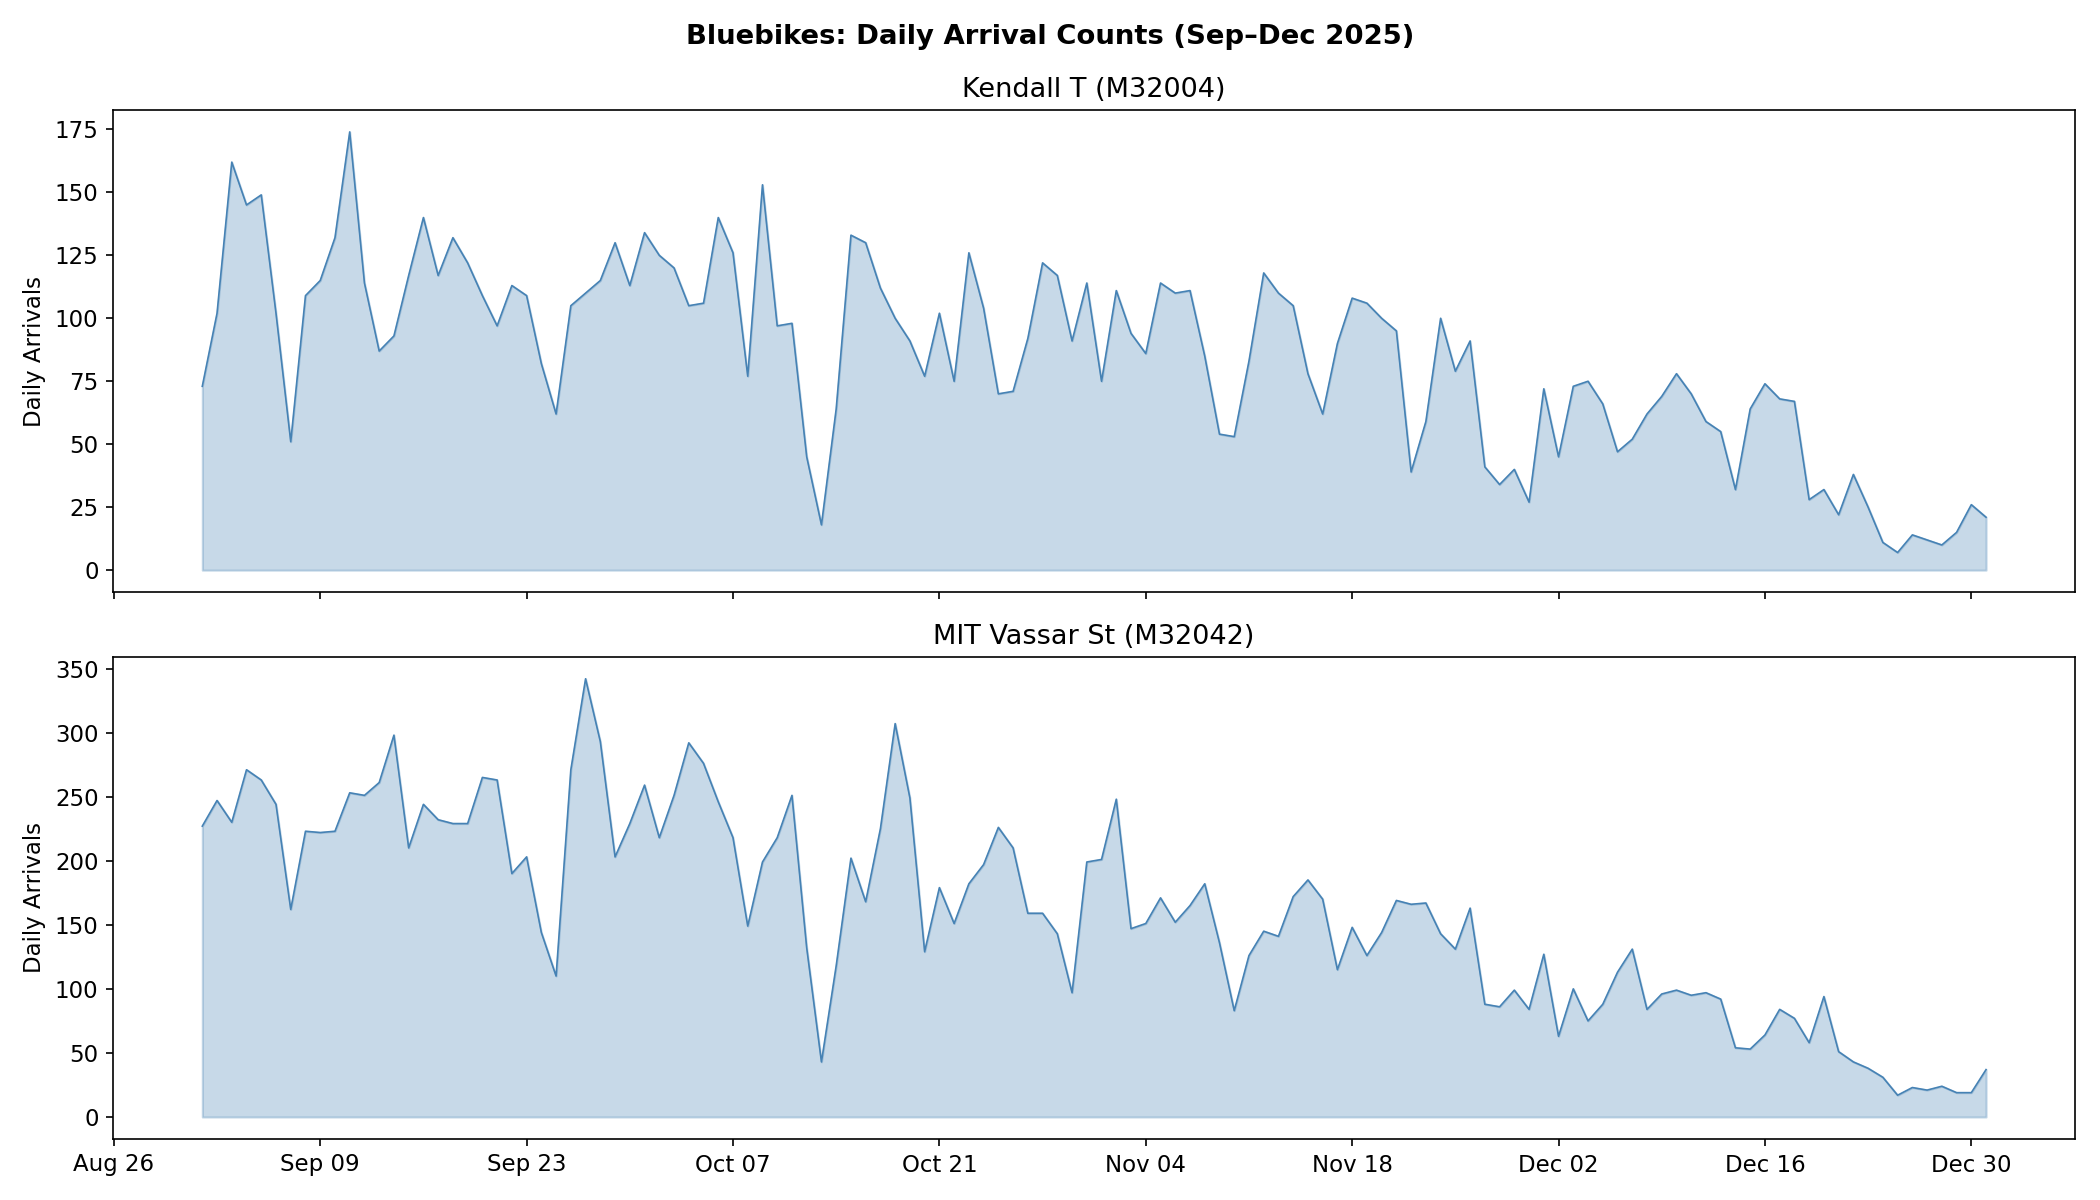
\includegraphics[width=\linewidth]{bb_daily_arrivals.png}
\caption{Bluebikes daily arrival counts at both stations, September--December 2025.}
\label{fig:bb-daily}
\end{figure}

\begin{figure}[h]
\centering
\begin{subfigure}{0.48\linewidth}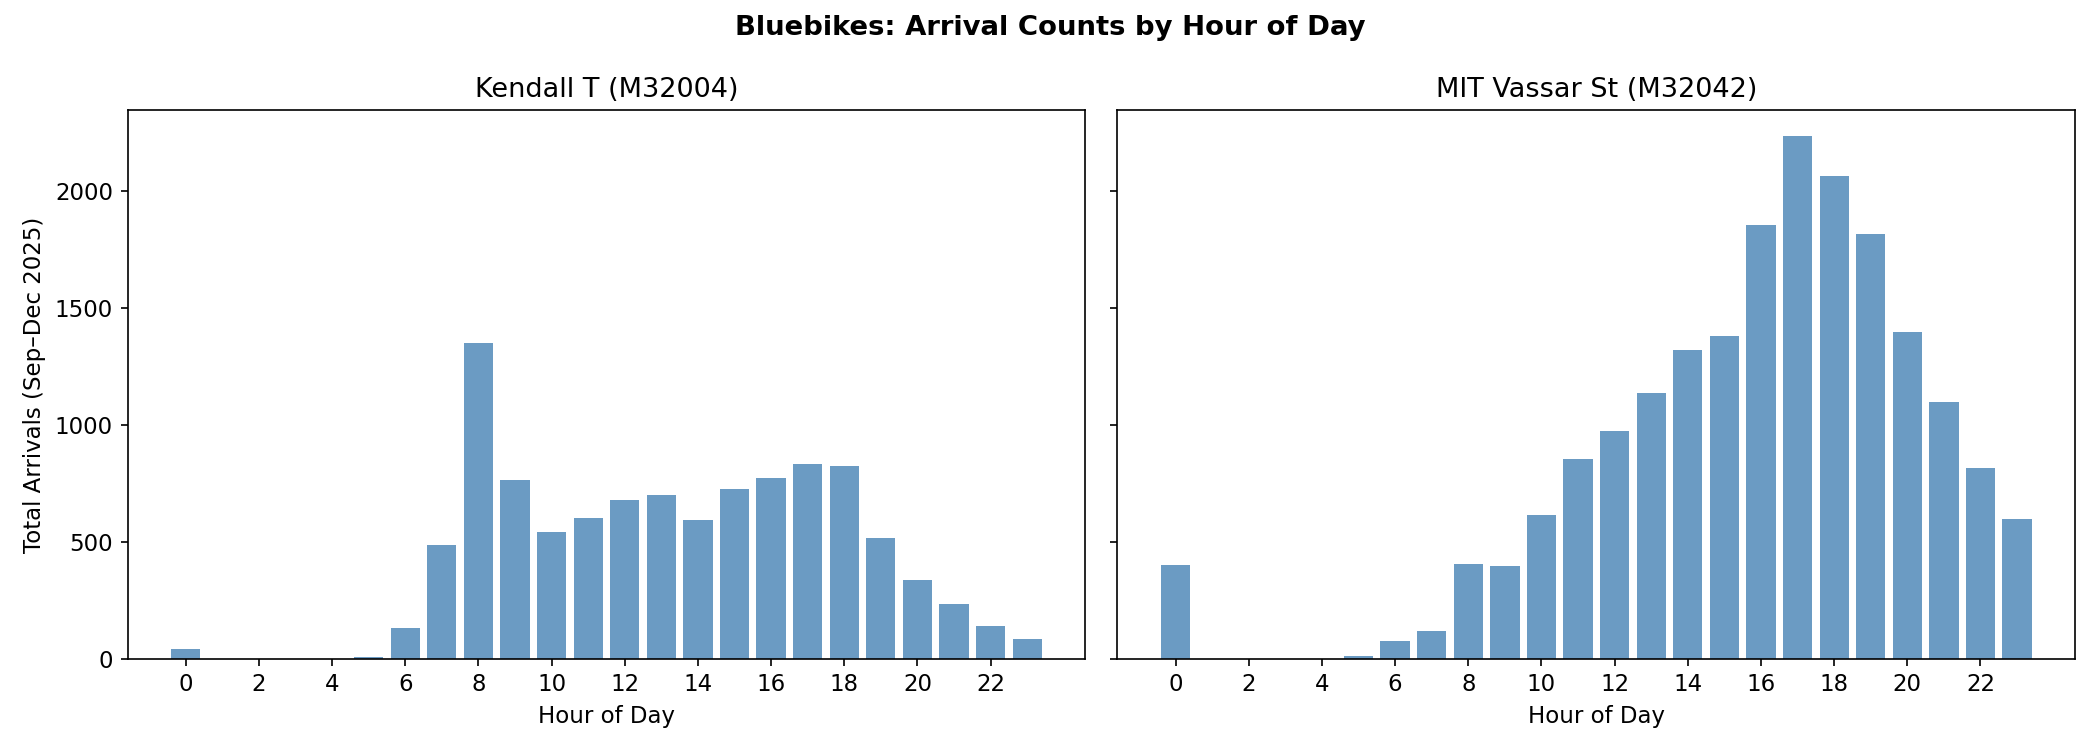
\includegraphics[width=\linewidth]{bb_arrivals_by_hour.png}\end{subfigure}
\hfill
\begin{subfigure}{0.48\linewidth}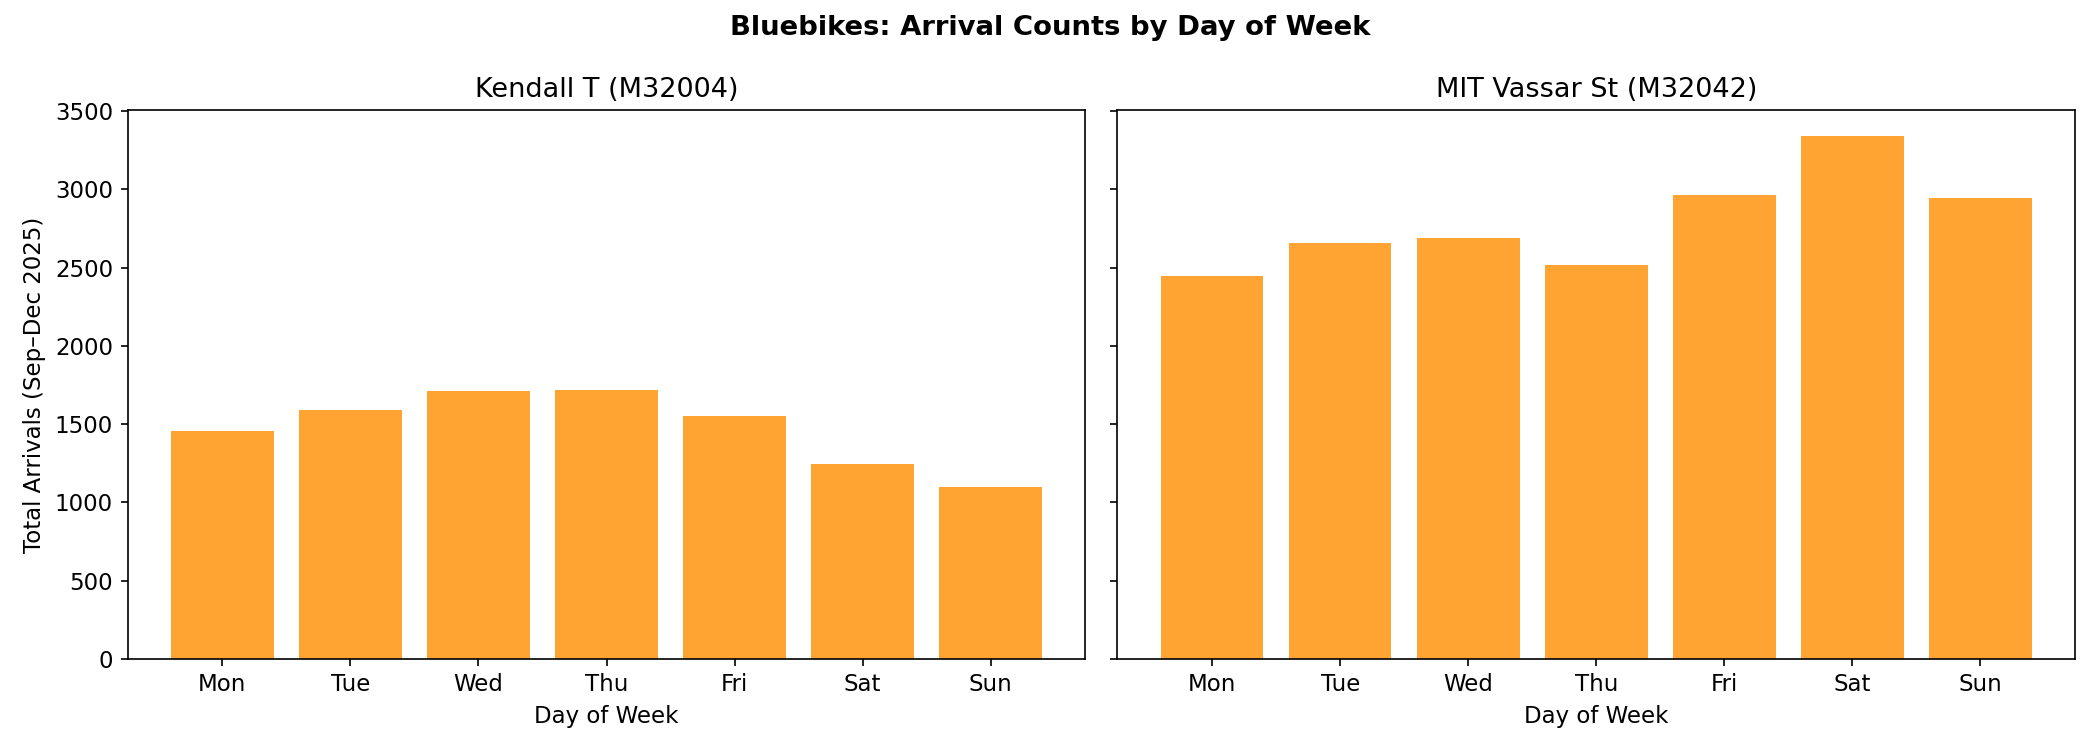
\includegraphics[width=\linewidth]{bb_arrivals_by_dow.png}\end{subfigure}
\caption{Bluebikes arrivals by hour-of-day (left) and by day-of-week (right).}
\label{fig:bb-seg}
\end{figure}

\begin{figure}[h]
\centering
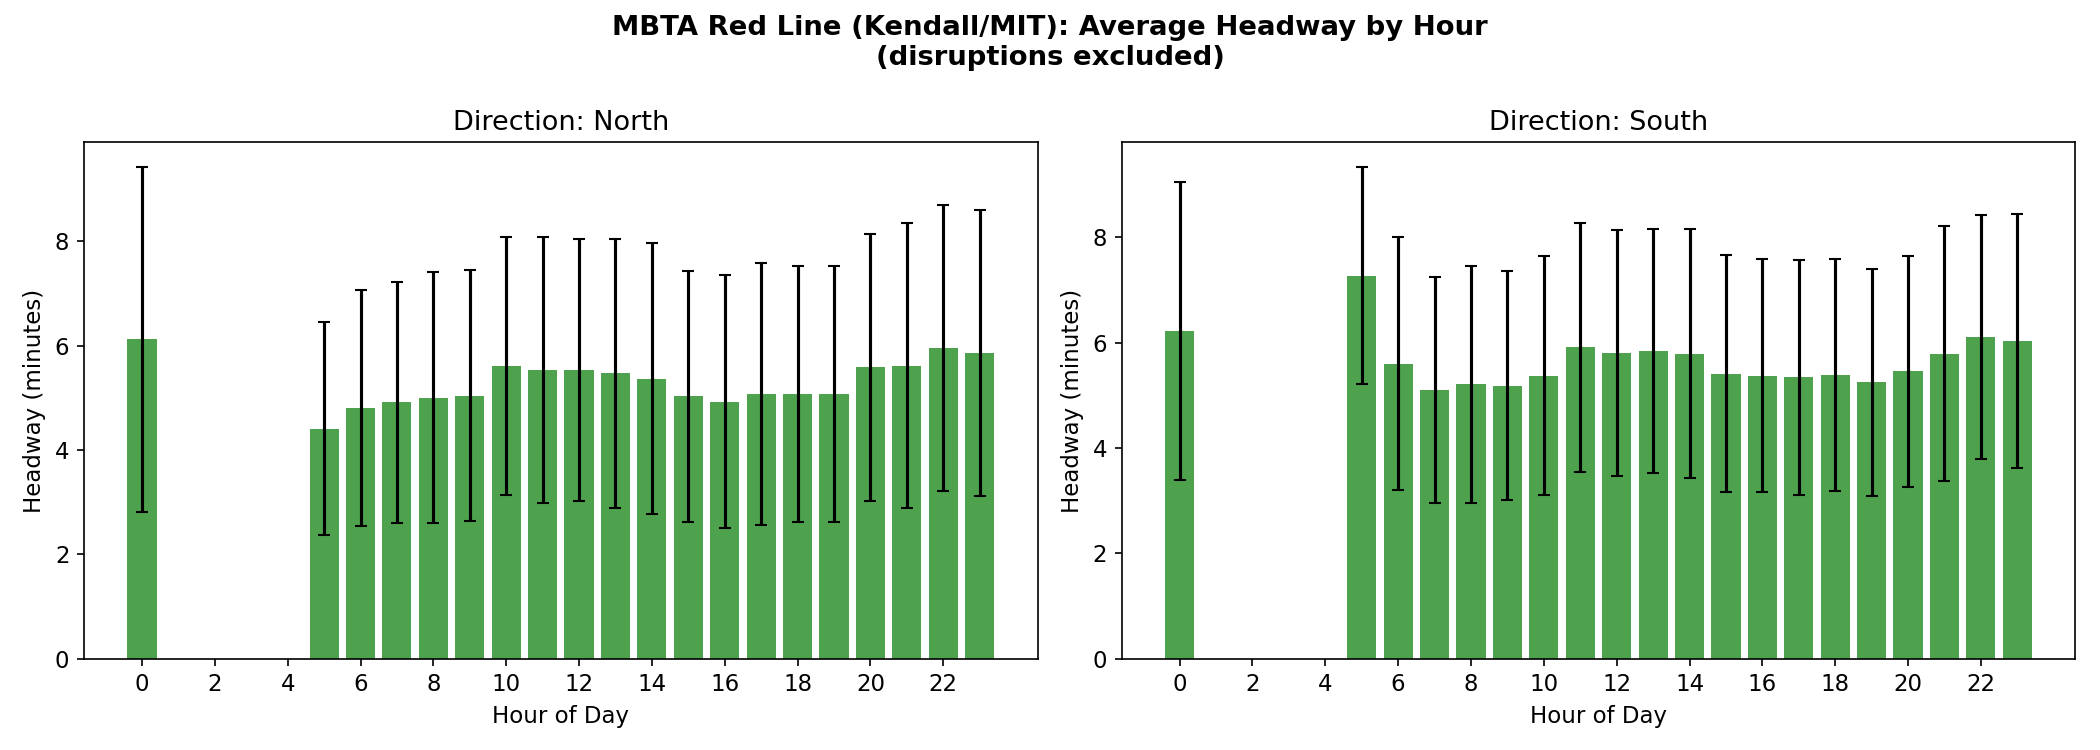
\includegraphics[width=0.7\linewidth]{mbta_headway_by_hour.png}
\caption{MBTA Red Line headway distribution by hour-of-day at Kendall/MIT.}
\label{fig:mbta-headway}
\end{figure}

\begin{figure}[h]
\centering
\begin{subfigure}{0.48\linewidth}
\includegraphics[width=\linewidth]{phase2_histograms.png}\end{subfigure}
\hfill
\begin{subfigure}{0.48\linewidth}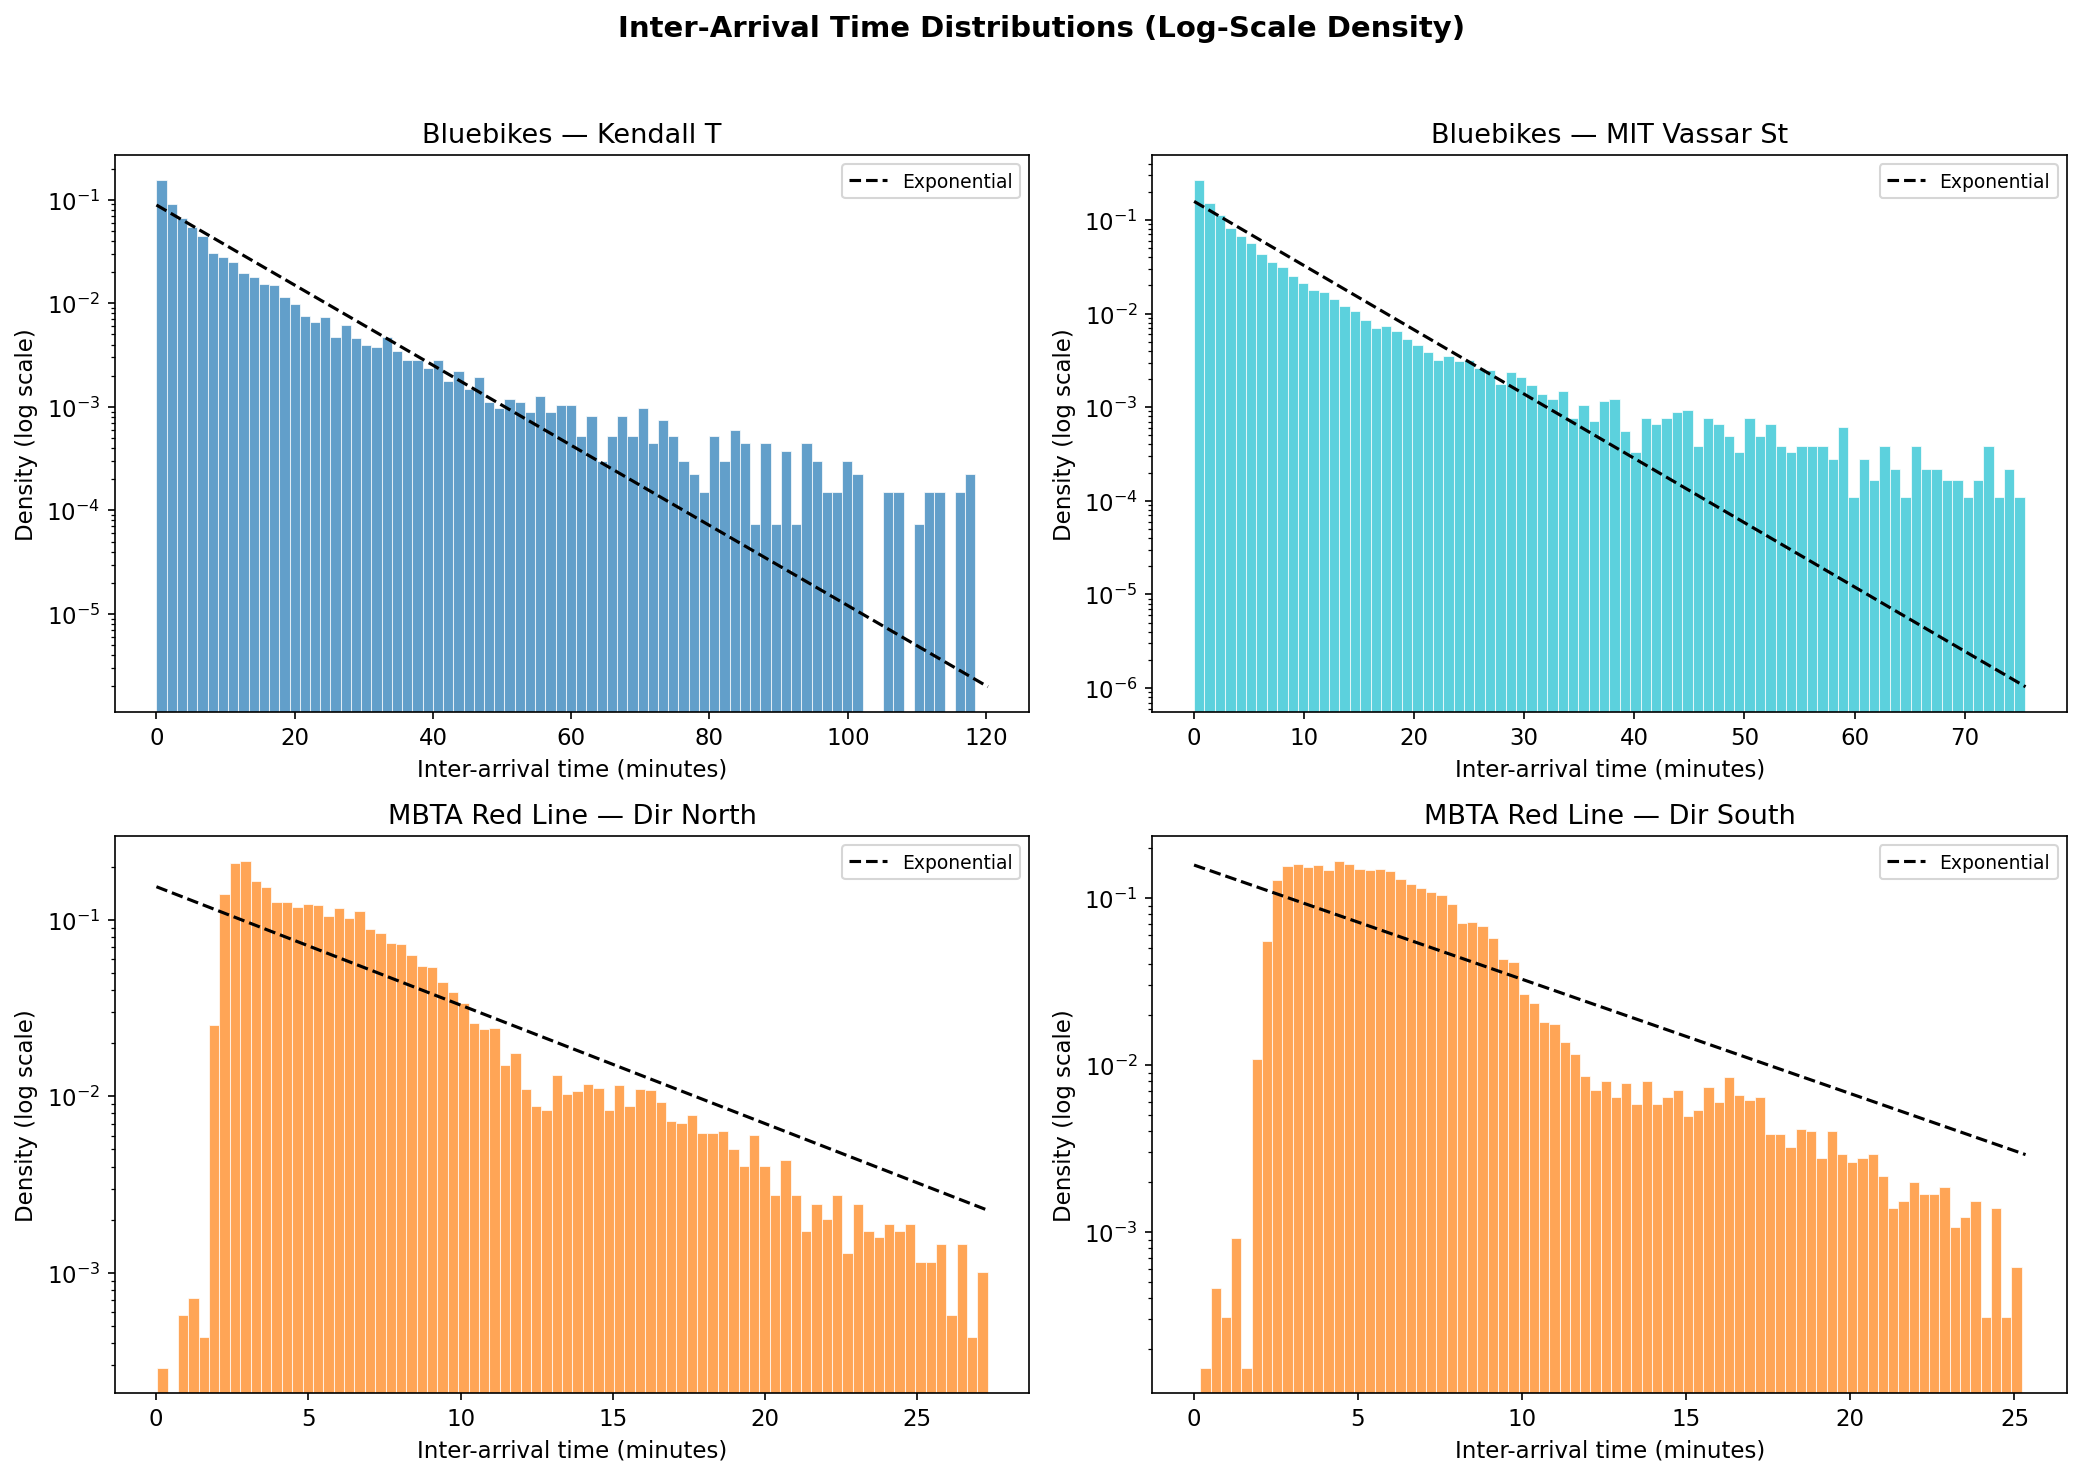
\includegraphics[width=\linewidth]{phase2_histograms_log.png}\end{subfigure}
\caption{IAT histograms with fitted distributions (linear and log scale).}
\label{fig:iat-hist}
\end{figure}

\begin{figure}[h]
\centering
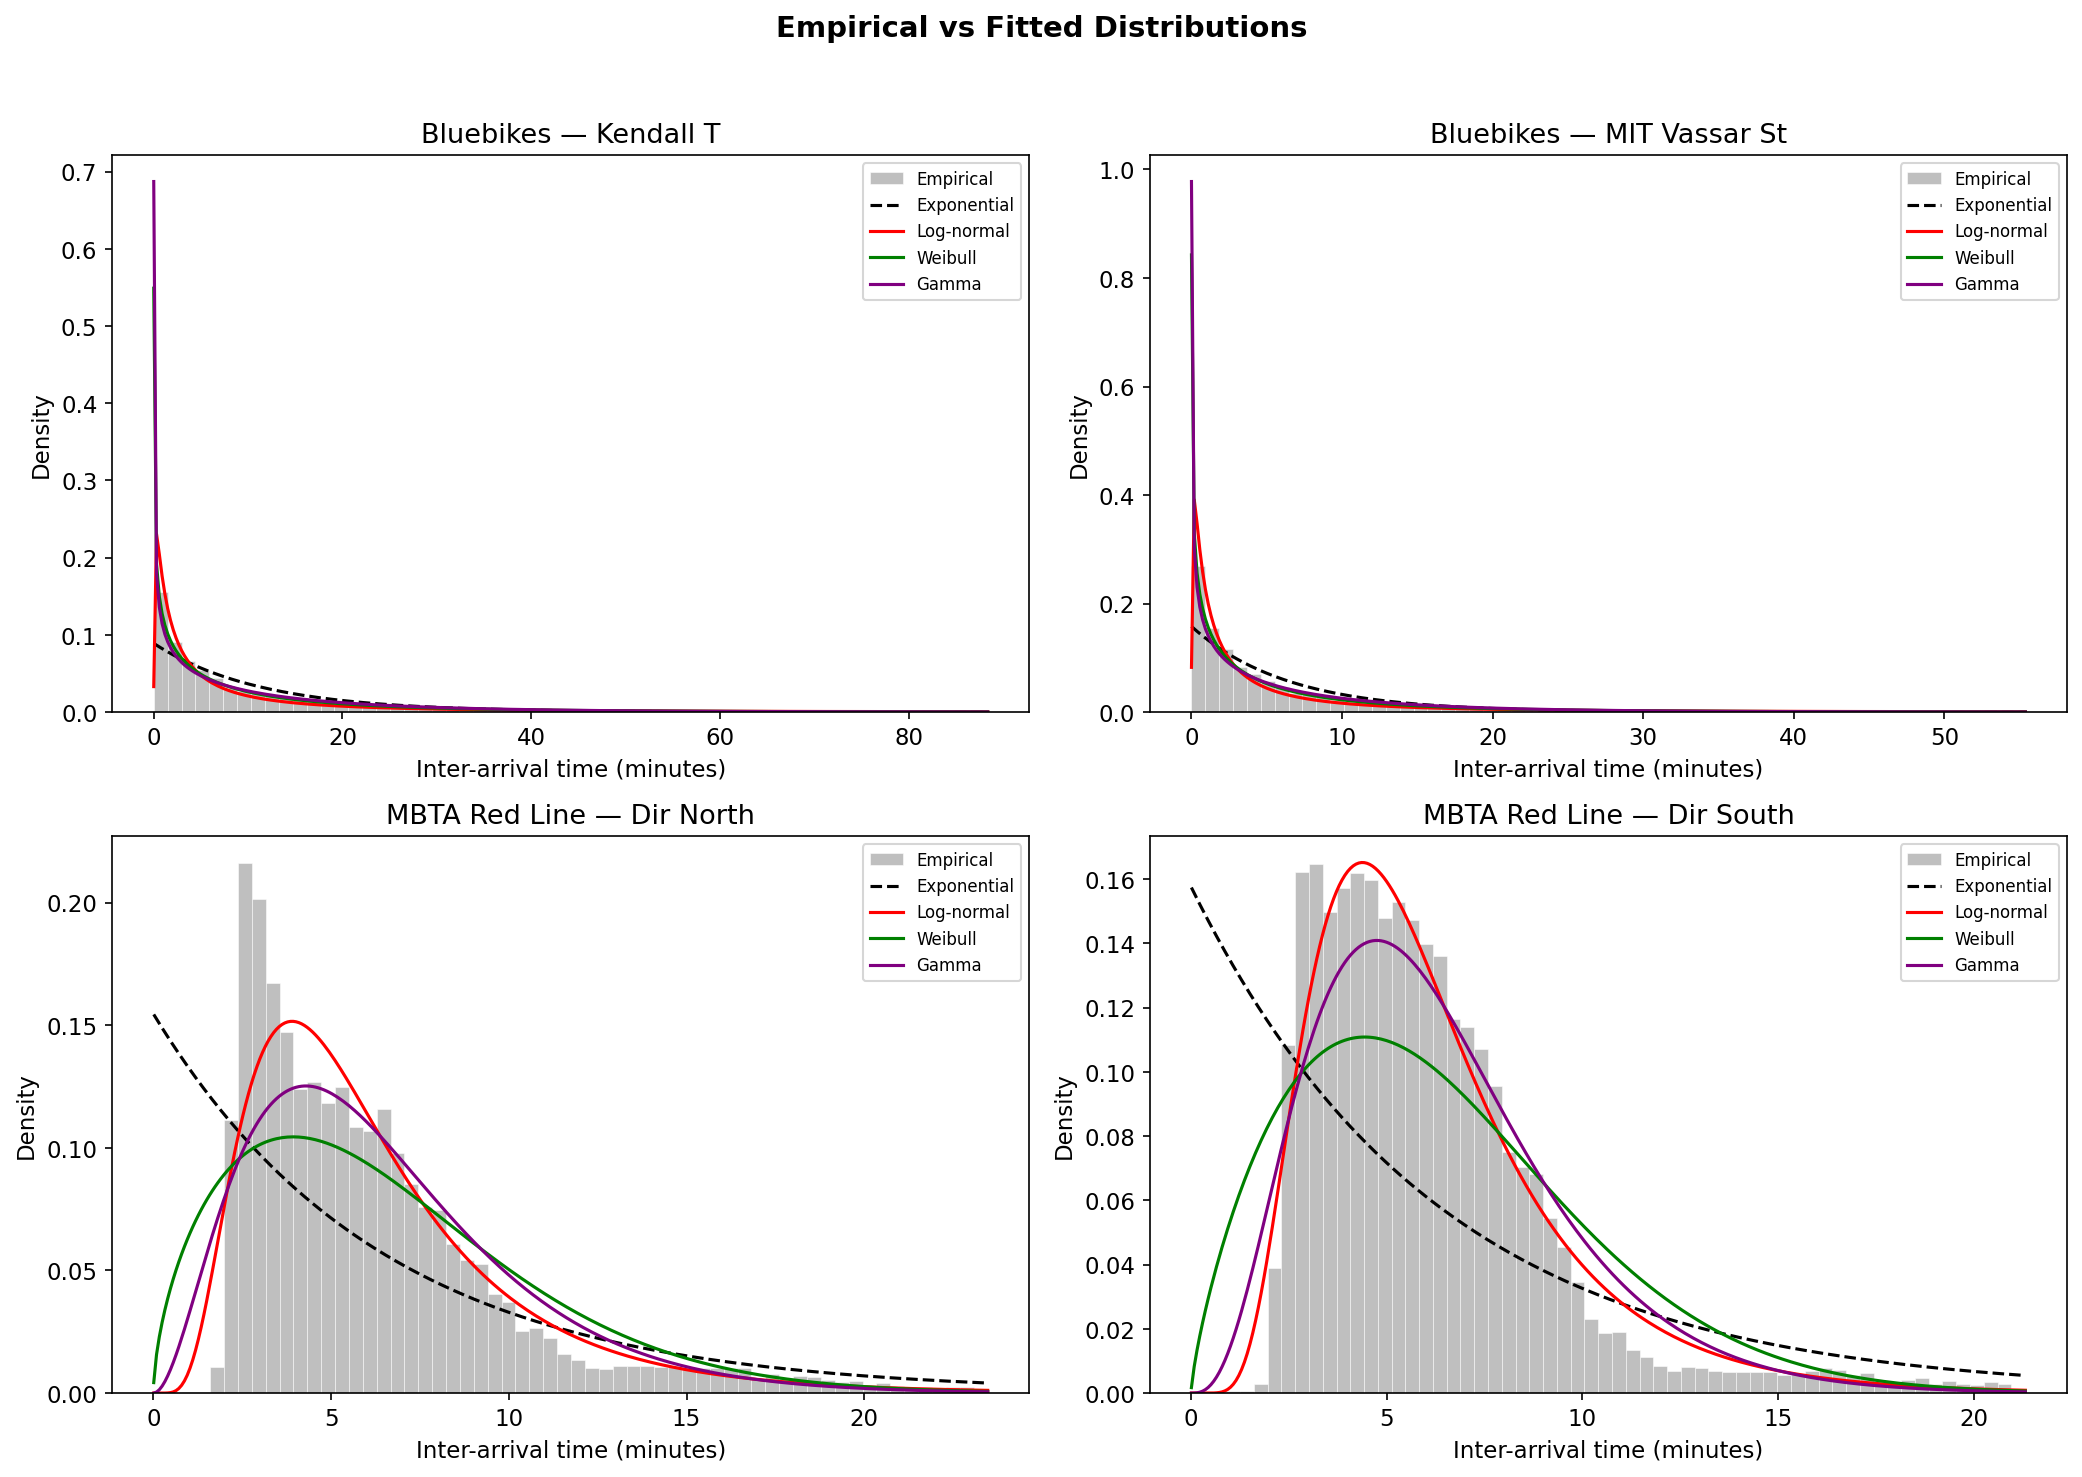
\includegraphics[width=\linewidth]{phase2_fitted_distributions.png}
\caption{Fitted distributions overlaid on empirical PDFs (Weibull best for Bluebikes; log-normal best for MBTA).}
\label{fig:fitted}
\end{figure}

\begin{figure}[h]
\centering
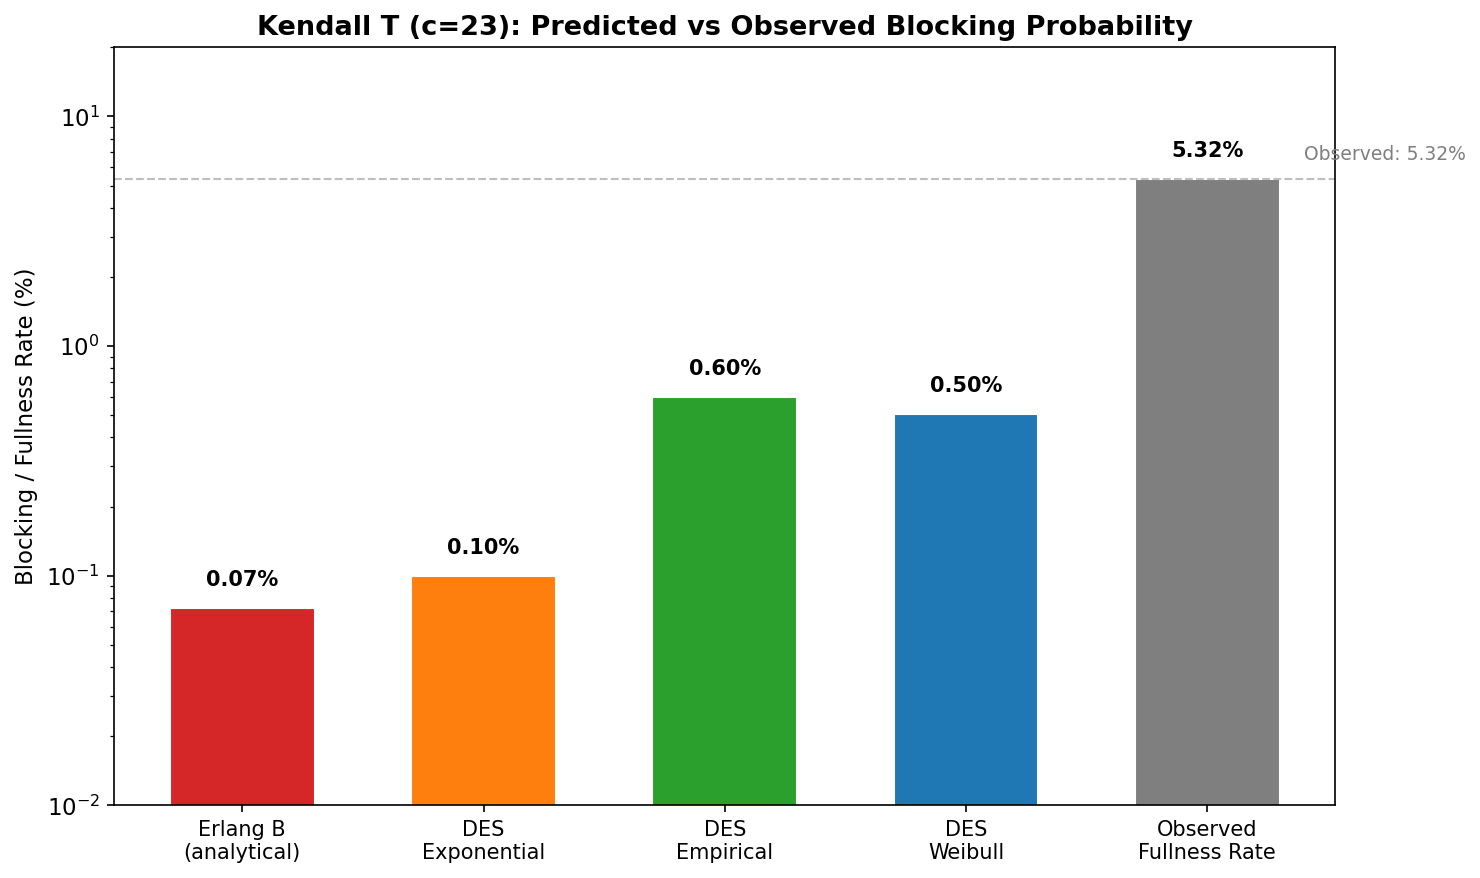
\includegraphics[width=0.75\linewidth]{phase3_blocking_comparison.png}
\caption{Blocking probability: Erlang B analytical vs.\ DES (Poisson) vs.\ DES (empirical) vs.\ observed full-capacity rate. Log $y$-axis. The 75$\times$ gap at Kendall/MIT is the visual centre.}
\label{fig:blocking}
\end{figure}

\begin{figure}[h]
\centering
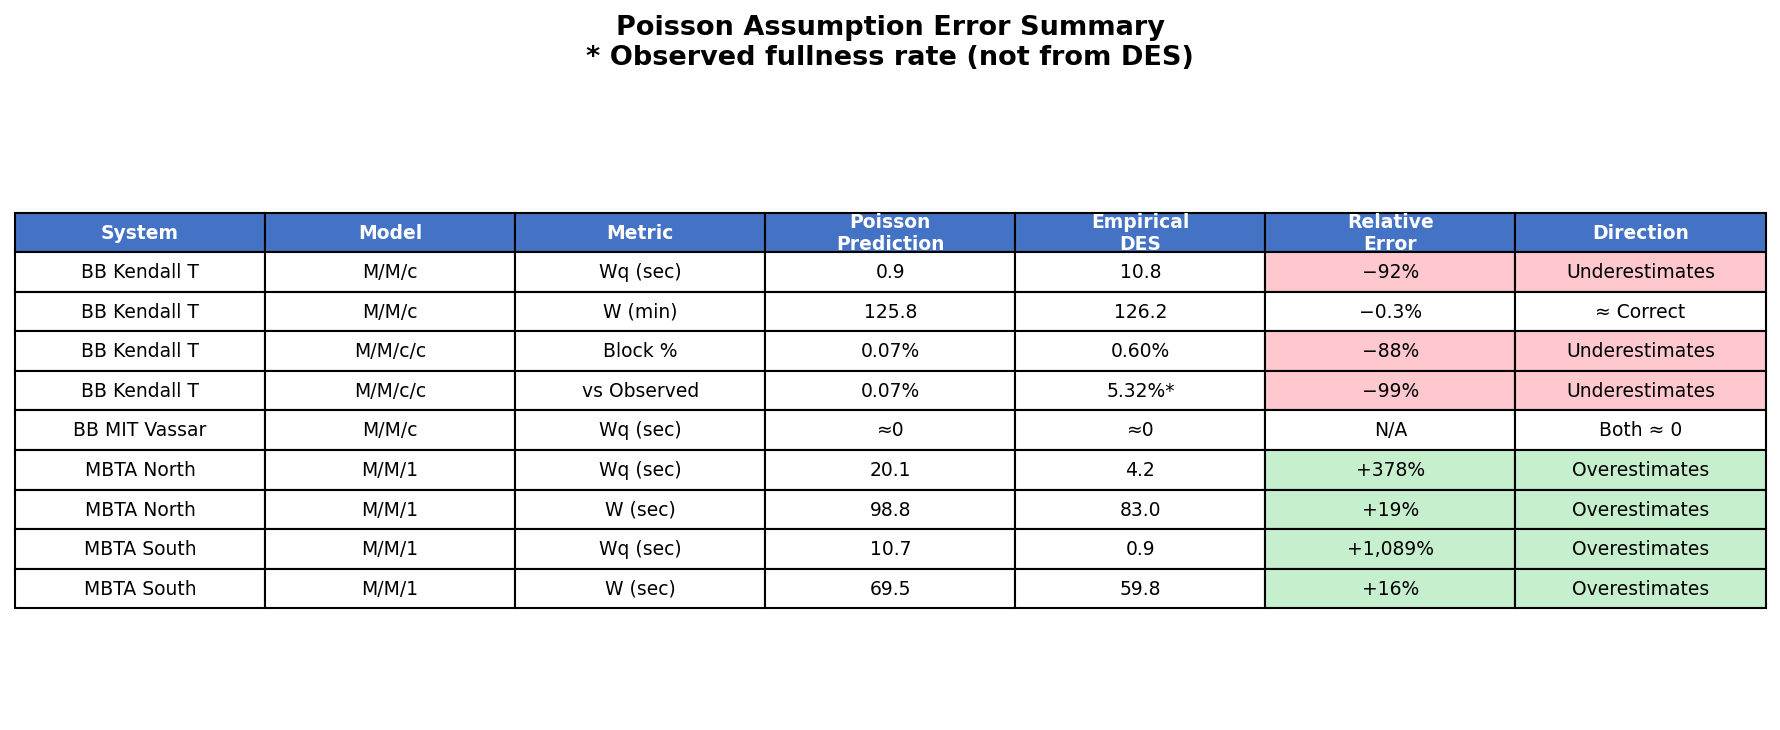
\includegraphics[width=0.9\linewidth]{phase3_error_summary.png}
\caption{Relative error of analytical Poisson predictions against empirical-DES benchmarks, across systems and metrics.}
\label{fig:error-summary}
\end{figure}

% ===== D. Derivations =====
\section{Derivations}\label{app:derivations}

\subsection{M/M/$c$ waiting time}\label{app:mmc}

Let $\lambda$ and $\mu$ denote the arrival rate and per-server service rate, $a = \lambda/\mu$, and $c$ the number of servers, with the stability requirement $\rho = a/c < 1$. The Erlang~C probability that an arrival finds all servers busy (and must queue) is
\begin{equation}
C(c, a) = \frac{\frac{a^c}{c!}\cdot\frac{1}{1-\rho}}{\sum_{k=0}^{c-1} \frac{a^k}{k!} + \frac{a^c}{c!}\cdot\frac{1}{1-\rho}}.
\end{equation}
Conditional on queueing, the residual wait in an M/M/$c$ system is exponential with rate $c\mu - \lambda$, so the unconditional expected wait is
\begin{equation}
W_q = \frac{C(c, a)}{c\mu - \lambda}.
\end{equation}
The expected queue length follows by Little's Law: $L_q = \lambda W_q$; and the expected system time is $W = W_q + 1/\mu$.

\subsection{Erlang B (M/M/$c/c$) blocking probability}\label{app:erlangb}

The finite-capacity M/M/$c/c$ model rejects any arrival that finds all servers busy. The stationary probability of rejection is the Erlang~B blocking formula
\begin{equation}
B(c, a) = \frac{a^c / c!}{\sum_{k=0}^{c} a^k / k!},
\end{equation}
which satisfies the numerically stable recursion
\begin{equation}
B(c, a) = \frac{a\,B(c-1, a)}{c + a\,B(c-1, a)}, \qquad B(0, a) = 1.
\end{equation}
We use the recursion throughout.

\subsection{Bluebikes service rate via Little's Law}\label{app:little}

Little's Law \cite{little1961} relates the mean number of entities in a stationary queueing system to the arrival rate and mean time spent: $L = \lambda W$. Applied to a single dock slot at station $s$ during non-full intervals, $L_{\text{slot}} = L_{\text{non-full}} / c$ is the mean occupancy fraction of a slot, $\lambda_{\text{slot}} = \lambda / c$ the per-slot arrival rate, and $W_{\text{slot}} = 1/\mu$ the mean service time. Rearranging,
\begin{equation}
\mu = \frac{\lambda / c}{L_{\text{non-full}} / c} = \frac{\lambda}{L_{\text{non-full}}}.
\end{equation}
This is a first-order estimate that treats all slots as exchangeable and conditions on non-full intervals to sidestep censoring. A more refined estimator would allow $\mu$ to vary by hour-of-day and is listed as future work (\S\ref{sec:future}).


\end{document}
